\documentclass[a4paper]{article}

\usepackage[a4paper,width=150mm,top=25mm,bottom=25mm]{geometry}
\usepackage[utf8x]{inputenc}
\usepackage{amsmath}
\usepackage{graphicx}

\title{INTL 450: Advanced Data Analysis in Python}
\author{Alper Yıldırım}

\begin{document}
\maketitle

\section{Homework 2: Report}

\subsection{Hypothesis and Analysis}
	In this homework assignment, I hypothesized that social assistance transfers predict life expectancy in Turkey. For my research purpose, I have compiled the life expectancy at birth data and average per capita transfer of all social assistance data of Turkey, using World Bank API. I applied \verb|linear_regress| function that I have written to data, taking life expectancy as dependent variable and average per capita transfer of all social assistance as independent variable. After excluding missing data through \verb|pandas.DataFrame.dropna()| function, the time interval remained limited between 2004 and 2018. Furthermore, because of the limitation of the scope, I have limited my focus only to all social assistance transfers. The regression results of this hypothesis is visualized with \verb|seaborn| module of Python and represented in Figure 1 below. Without a constant $\beta_0$, the regression coefficient $\beta_1$ is equal to 143.68, which demonstrates a apparent causal relationship between social assistance transfers and life expectancy. In further studies, the effects of different types of social assistance transfers can be investigated. Furthermore, the causal effect of social assistance transfers on life expectancy should be examined for different income quintiles, since the lower income groups receive more social assistance.

\begin{figure}[htp]
    \centering
    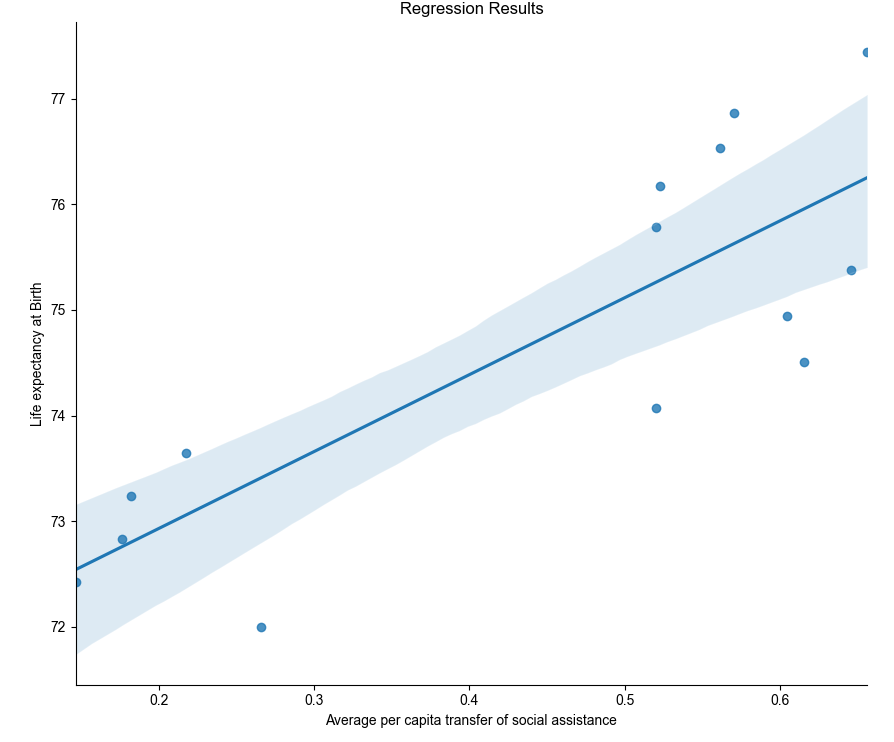
\includegraphics[width=10cm]{RegressionResults.png}
    \caption{Regression Results}
\end{figure}

\subsection{Bonus}
    I have used STATA Software to make a comparison with my regression results. I have passed \verb|noconstant| argument in STATA, since the \verb|linear_regress| function I have written does not include any $\beta_0$ values. Both the output of \verb|linear_regress| and STATA Software have the same regression coefficient: 143.6813. Standard errors of \verb|linear_regress| and STATA Software are almost equal, 16.82 for \verb|linear_regress| and 16.16 for STATA output. However, in the 95\% Confidence Interval, there is a non-negligible discrepancy. In \verb|linear_regress|, the CI is (110.70, 176.66) whereas in STATA Software, it is (108.76, 178.60). The reason of this discrepancy might be that I have used 1.96 as Z-Score as constant for the calculation of the CI, however, the STATA Software might have used more complex method to determine t-statistic.

\end{document}